\chapter{Osteoarthritis of the Knee}
\label{applications-con_fit_splines}

Osteoarthritis (OA) is a degenerative disease of joints. The hip and knee are the common sites of OA in the larger joints.

    \begin{figure}[h]
        \begin{center}
            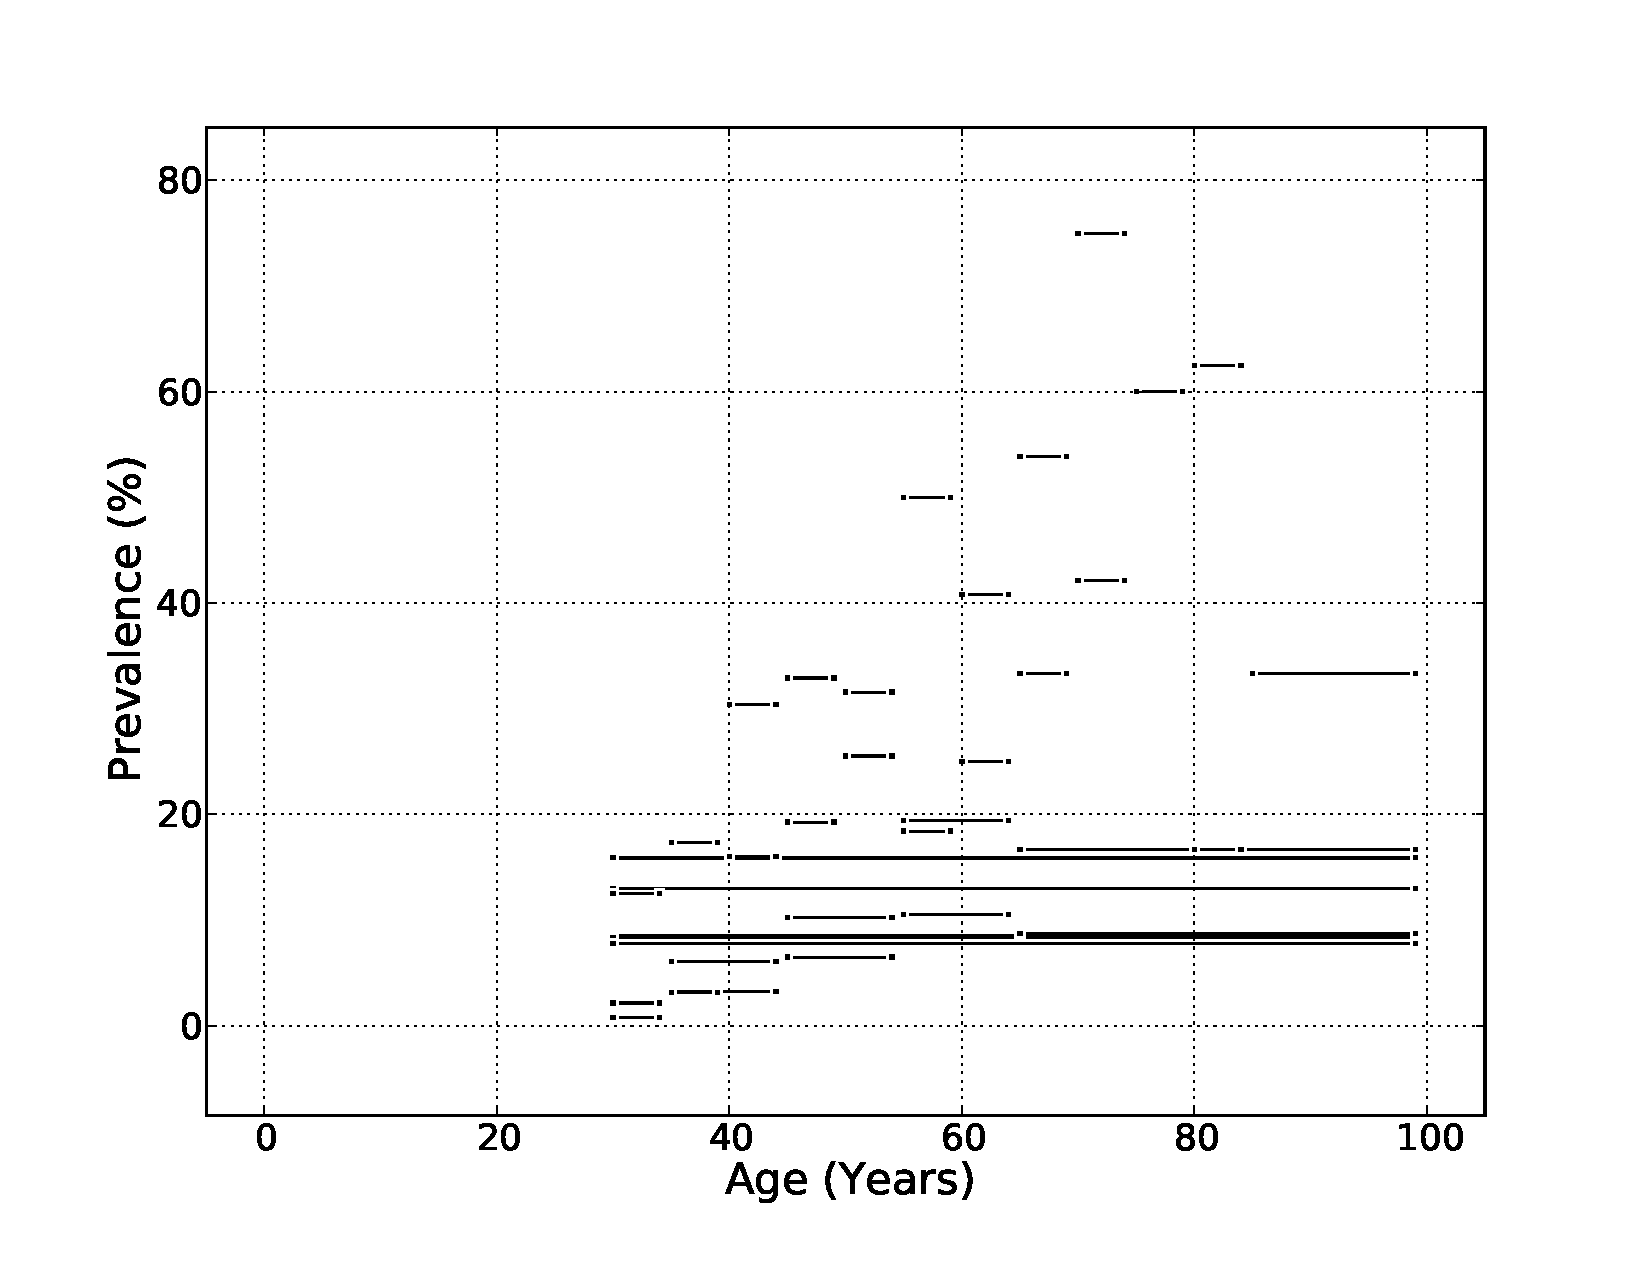
\includegraphics[width=\textwidth]{oa_knee-data.pdf}
            \caption{Prevalence data from systematic review included for the modeling of osteoarthritis of the knee in females in South Asia.}
            \label{fig:app-oa knee data}
        \end{center}
    \end{figure}

    \begin{figure}[h]
        \begin{center}
            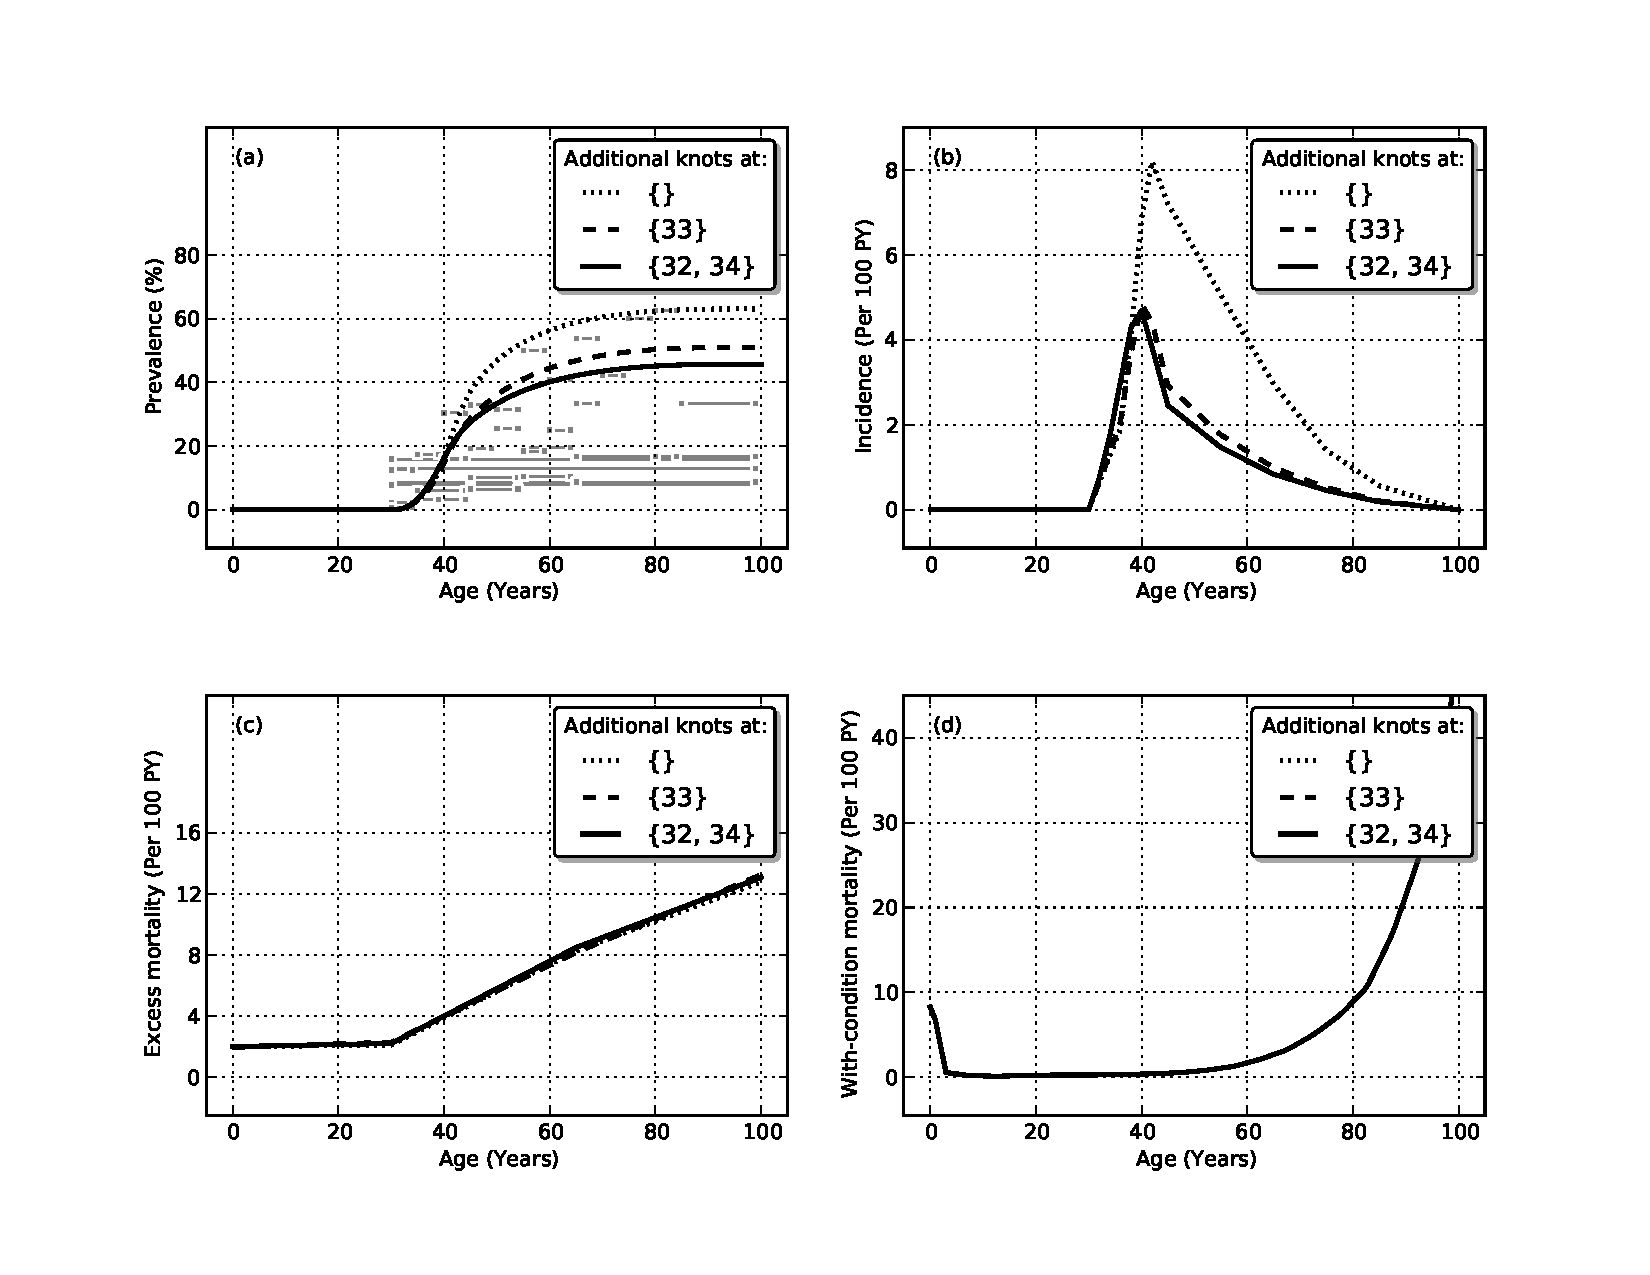
\includegraphics[width=\textwidth]{oa_knee-knots.pdf}
            \caption{female South Asia 2005  All models have knots at age {0, 30, 100}.  40, 35, 31.}
            \label{fig:app-oa knee knots}
        \end{center}
    \end{figure}

    \begin{figure}[h]
        \begin{center}
            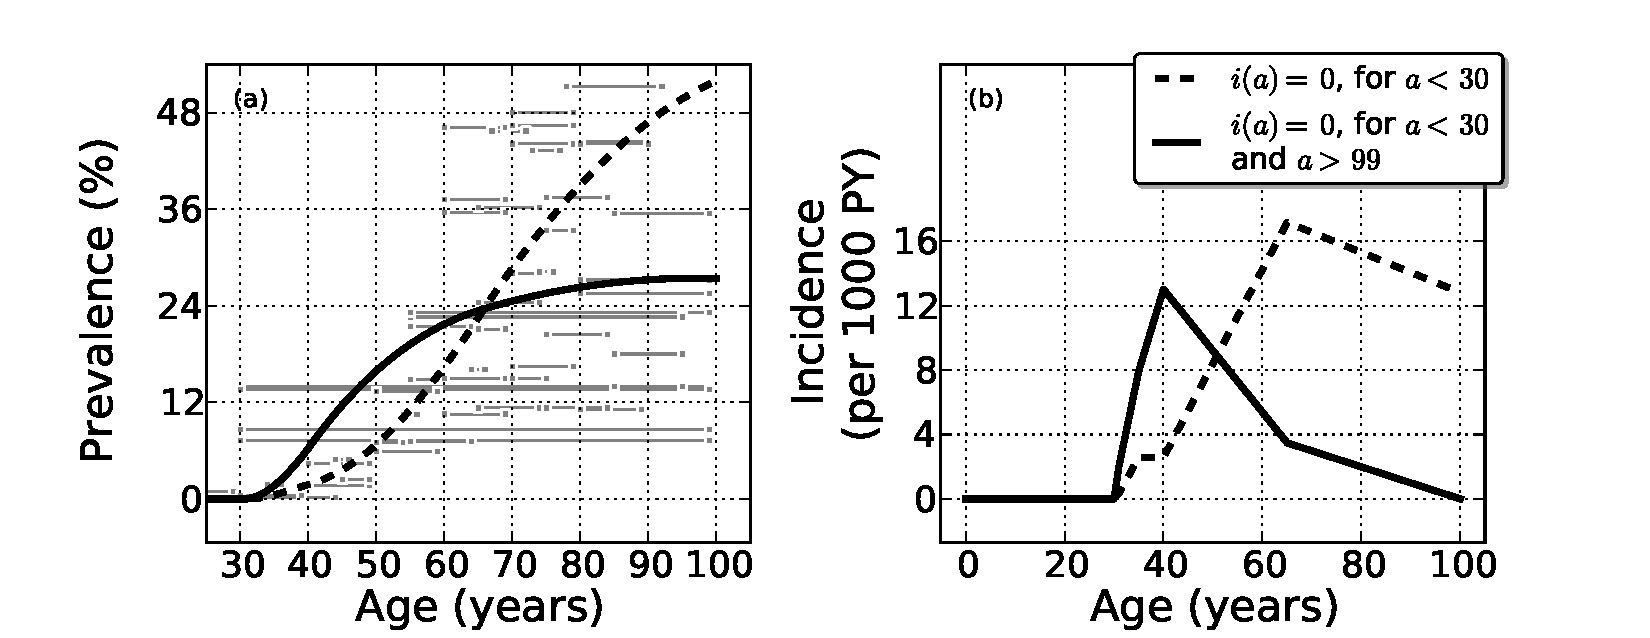
\includegraphics[width=\textwidth]{oa_knee-i_prior.pdf}
            \caption{female South Asia 2005.}
            \label{fig:app-oa knee knots}
        \end{center}
    \end{figure} 